\documentclass[tikz,border=10pt]{standalone}
% Trapezoid ABCD with diagonal BD; no circles, no right-angle marks.
% Repair: edges and diagonal BD raised to 1.6pt; vertex labels enlarged and bolded (positions unchanged).
\begin{document}
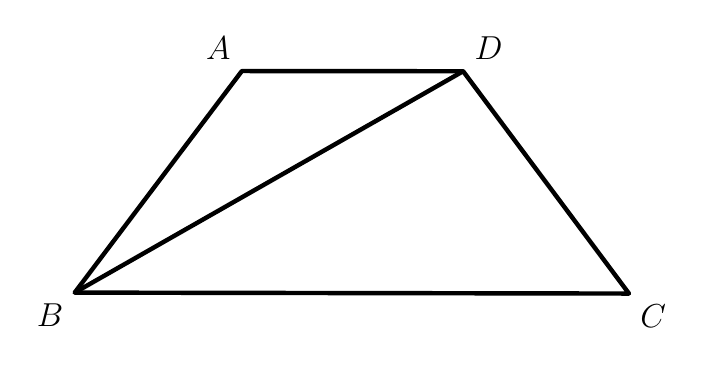
\begin{tikzpicture}[line join=round, line width=1.6pt]
  % Vertices: px -> units with s=0.014953, cx=305.5, cy=160.5, y flipped
  \coordinate (A) at (-1.398,  1.428);
  \coordinate (B) at (-3.521, -1.386);
  \coordinate (C) at ( 3.518, -1.398);
  \coordinate (D) at ( 1.412,  1.425);

  % Solid edges of the quadrilateral (1.6pt)
  \draw (A) -- (B) -- (C) -- (D) -- cycle;

  % Diagonal BD (solid, 1.6pt)
  \draw (B) -- (D);

  % Labels placed outside the figure; larger and bold
  \node[above left,  font=\large\bfseries] at (A) {$A$};
  \node[above right, font=\large\bfseries] at (D) {$D$};
  \node[below left,  font=\large\bfseries] at (B) {$B$};
  \node[below right, font=\large\bfseries] at (C) {$C$};
\end{tikzpicture}
\end{document}